% KADD pipeline figure: precompute -> data loading/caching -> cnn3d-light
% architecture -> pos_weight loss weighting.
%
% Compile with:  tectonic pipeline_figure.tex     (or pdflatex/xelatex)
%
% All facts in this figure are taken directly from the current source:
%   kadd/classify/data.py       (load_series_volume, KneeDataset, cache)
%   kaggle_kernel_precompute/precompute_kernel.py
%   scripts/kaggle_push_precomputed_dataset.py
%   kadd/classify/model.py      (CNN3D_CHANNELS['light'], SeriesMetaEmbed,
%                                 GatedAttentionMIL, KneeClassifier)
%   kadd/classify/train.py      (_compute_pos_weight, train_epoch/val_epoch)
%   config_files/classify_cnn3d_light.yml

\documentclass[border=8pt]{standalone}
\usepackage{tikz}
\usepackage{amsmath}
\usetikzlibrary{positioning, arrows.meta, fit, shapes.geometric, backgrounds, calc}

\begin{document}
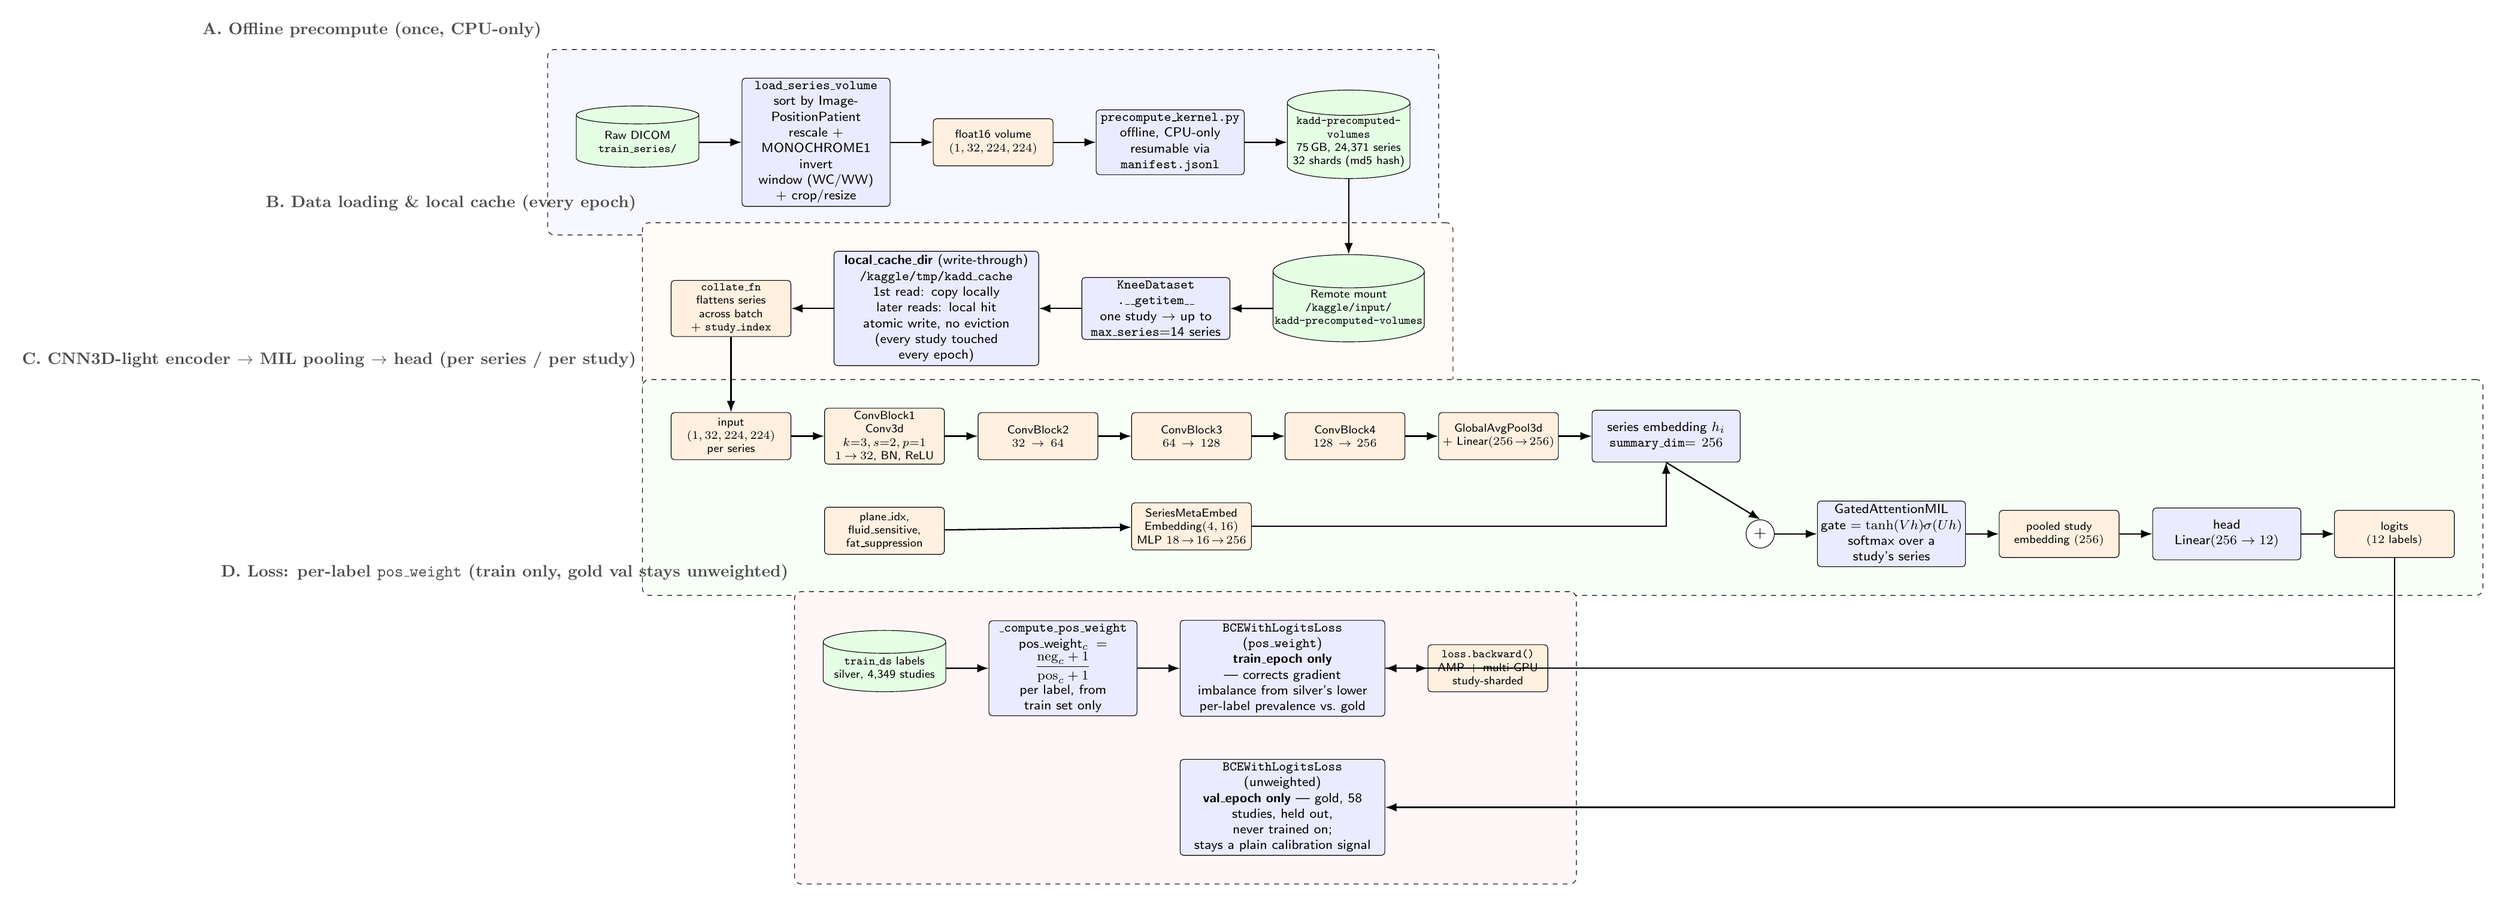
\begin{tikzpicture}[
  font=\sffamily,
  block/.style={draw, rounded corners=2pt, fill=blue!8, align=center,
                text width=30mm, minimum height=11mm, inner sep=2pt, font=\footnotesize\sffamily},
  small/.style={draw, rounded corners=2pt, fill=orange!12, align=center,
                text width=24mm, minimum height=10mm, inner sep=2pt, font=\scriptsize\sffamily},
  wide/.style={draw, rounded corners=2pt, fill=blue!8, align=center,
                text width=42mm, minimum height=11mm, inner sep=2pt, font=\footnotesize\sffamily},
  data/.style={draw, cylinder, shape border rotate=90, aspect=0.22, fill=green!10,
               align=center, font=\scriptsize\sffamily, minimum height=13mm, minimum width=26mm,
               inner sep=1pt},
  merge/.style={draw, circle, fill=white, minimum size=6mm, inner sep=0pt, font=\bfseries},
  arr/.style={-{Latex[length=2.4mm,width=1.8mm]}, thick},
  stagetag/.style={font=\bfseries\normalsize, anchor=west, text=black!70},
  >=Latex,
]

% ============================== STAGE A: PRECOMPUTE (offline) ==============
\node[data]                       (a1) {Raw DICOM\\\texttt{train\_series/}};
\node[block, right=9mm of a1]     (a2) {\texttt{load\_series\_volume}\\
                                          sort by ImagePositionPatient\\
                                          rescale + MONOCHROME1 invert\\
                                          window (WC/WW) + crop/resize};
\node[small, right=9mm of a2]     (a3) {float16 volume\\$(1,32,224,224)$};
\node[block, right=9mm of a3]     (a4) {\texttt{precompute\_kernel.py}\\
                                          offline, CPU-only\\
                                          resumable via \texttt{manifest.jsonl}};
\node[data, right=9mm of a4]      (a5) {\texttt{kadd-precomputed-}\\\texttt{volumes}\\
                                          75\,GB, 24{,}371 series\\32 shards (md5 hash)};

\draw[arr] (a1) -- (a2);
\draw[arr] (a2) -- (a3);
\draw[arr] (a3) -- (a4);
\draw[arr] (a4) -- (a5);

% ============================== STAGE B: DATA LOADING + CACHE ==============
\node[data,  below=16mm of a5]    (b1) {Remote mount\\\texttt{/kaggle/input/}\\
                                          \texttt{kadd-precomputed-volumes}};
\node[block, left=9mm of b1]      (b2) {\texttt{KneeDataset}\\\texttt{.\_\_getitem\_\_}\\
                                          one study $\to$ up to\\\texttt{max\_series}=14 series};
\node[wide,  left=9mm of b2]      (b3) {\textbf{local\_cache\_dir} (write-through)\\
                                          \texttt{/kaggle/tmp/kadd\_cache}\\
                                          1st read: copy locally\\ later reads: local hit\\
                                          atomic write, no eviction\\
                                          (every study touched every epoch)};
\node[small, left=9mm of b3]      (b4) {\texttt{collate\_fn}\\flattens series\\across batch\\
                                          $+$ \texttt{study\_index}};

\draw[arr] (a5) -- (b1);
\draw[arr] (b1) -- (b2);
\draw[arr] (b2) -- (b3);
\draw[arr] (b3) -- (b4);

% ============================== STAGE C: CNN3D-LIGHT ENCODER ================
\node[small, below=16mm of b4]    (c0) {input\\$(1,32,224,224)$\\per series};
\node[small, right=7mm of c0]     (c1) {ConvBlock1\\Conv3d $k{=}3,s{=}2,p{=}1$\\$1\!\to\!32$, BN, ReLU};
\node[small, right=7mm of c1]     (c2) {ConvBlock2\\$32\!\to\!64$};
\node[small, right=7mm of c2]     (c3) {ConvBlock3\\$64\!\to\!128$};
\node[small, right=7mm of c3]     (c4) {ConvBlock4\\$128\!\to\!256$};
\node[small, right=7mm of c4]     (c5) {GlobalAvgPool3d\\$+$ Linear$(256\!\to\!256)$};
\node[block, right=7mm of c5]     (c6) {series embedding $h_i$\\\texttt{summary\_dim}$=256$};

\draw[arr] (c0) -- (c1);
\draw[arr] (c1) -- (c2);
\draw[arr] (c2) -- (c3);
\draw[arr] (c3) -- (c4);
\draw[arr] (c4) -- (c5);
\draw[arr] (c5) -- (c6);

\node[small, below=9mm of c1]     (cm1) {plane\_idx,\\fluid\_sensitive,\\fat\_suppression};
\node[small, below=9mm of c3]     (cm2) {SeriesMetaEmbed\\Embedding$(4,16)$\\MLP $18\!\to\!16\!\to\!256$};

\draw[arr] (cm1) -- (cm2);
\draw[arr] (cm2.east) -| ($(c6.south)+(0,-6mm)$) -- (c6.south);

\node[merge, below right=13mm and 2mm of c6] (plus) {$+$};
\node[block, right=9mm of plus]   (c7) {GatedAttentionMIL\\
                                          gate $=\tanh(Vh)\!\cdot\!\sigma(Uh)$\\
                                          softmax over a study's series};
\node[small, right=7mm of c7]     (c8) {pooled study\\embedding $(256)$};
\node[block, right=7mm of c8]     (c9) {head\\Linear$(256\!\to\!12)$};
\node[small, right=7mm of c9]     (c10) {logits\\$(12$ labels$)$};

\draw[arr] (c6.south) -- (plus.north);
\draw[arr] (plus) -- (c7);
\draw[arr] (c7) -- (c8);
\draw[arr] (c8) -- (c9);
\draw[arr] (c9) -- (c10);

\draw[arr] (b4.south) -| ($(c0.north)+(0,6mm)$) -- (c0.north);

% ============================== STAGE D: LOSS (pos_weight) ==================
\node[data,  below=16mm of cm1]   (d1) {\texttt{train\_ds} labels\\silver, 4{,}349 studies};
\node[block, right=9mm of d1]     (d2) {\texttt{\_compute\_pos\_weight}\\
                                          pos\_weight$_c=\dfrac{\mathrm{neg}_c+1}{\mathrm{pos}_c+1}$\\
                                          per label, from train set only};
\node[wide,  right=9mm of d2]     (d3) {\texttt{BCEWithLogitsLoss}\\(\texttt{pos\_weight})\\
                                          \textbf{train\_epoch only} --- corrects gradient\\
                                          imbalance from silver's lower\\
                                          per-label prevalence vs.\ gold};
\node[wide,  below=9mm of d3]     (d4) {\texttt{BCEWithLogitsLoss}\\(unweighted)\\
                                          \textbf{val\_epoch only} --- gold, 58\\
                                          studies, held out, never trained on;\\
                                          stays a plain calibration signal};
\node[small, right=9mm of d3]     (d5) {\texttt{loss.backward()}\\AMP $+$ multi-GPU\\study-sharded};

\draw[arr] (d1) -- (d2);
\draw[arr] (d2) -- (d3);
\draw[arr] (c10.south) |- (d3.east);
\draw[arr] (c10.south) |- (d4.east);
\draw[arr] (d3) -- (d5);

% ============================== stage backgrounds + labels ==================
\begin{pgfonlayer}{background}
  \node[fit=(a1)(a2)(a3)(a4)(a5), draw, dashed, rounded corners=4pt,
        fill=blue!3, inner sep=6mm] (boxA) {};
  \node[fit=(b1)(b2)(b3)(b4), draw, dashed, rounded corners=4pt,
        fill=orange!3, inner sep=6mm] (boxB) {};
  \node[fit=(c0)(c1)(c2)(c3)(c4)(c5)(c6)(cm1)(cm2)(plus)(c7)(c8)(c9)(c10),
        draw, dashed, rounded corners=4pt, fill=green!3, inner sep=6mm] (boxC) {};
  \node[fit=(d1)(d2)(d3)(d4)(d5), draw, dashed, rounded corners=4pt,
        fill=red!3, inner sep=6mm] (boxD) {};
\end{pgfonlayer}

\node[stagetag, above left=1mm and 0mm of boxA.north west] {A. Offline precompute (once, CPU-only)};
\node[stagetag, above left=1mm and 0mm of boxB.north west] {B. Data loading \& local cache (every epoch)};
\node[stagetag, above left=1mm and 0mm of boxC.north west] {C. CNN3D-light encoder $\to$ MIL pooling $\to$ head (per series / per study)};
\node[stagetag, above left=1mm and 0mm of boxD.north west] {D. Loss: per-label \texttt{pos\_weight} (train only, gold val stays unweighted)};

\end{tikzpicture}
\end{document}
